\chapter{Testovanie a vyhodnocovanie}
\label{chap:testovanie-vyhodnocovanie}
Po naimplementovaní navrhnutého riešenia, ktoré bolo popísané v kapitole \ref{chap:implementacia}, nasledovalo testovanie a vyhodnocovanie, ktorému sa venuje práve táto kapitola.  Kapitola začína popisom testovania serverového aplikačného riešenia pomocou testovacieho rámca Tavern, pokračuje testovaním užívateľského rozhrania aplikácie a vyhodnocovaním naimplementovanej detekcie chronických rán. Na záver kapitoly sú zhrnuté ďalšie možné vylepšenia práce a je načrtnuté budúce smerovanie projektu. 

%%%%%%%%%%%%%%%%%%%%%%%%%%%%%%%%%%%%%%%%%%%%%%%%%%%%%%%%%%%%%%
\section{Testovanie serverového aplikačného rozhrania}
Testovanie aplikačného rozhrania prebiehalo už počas samotnej implementácie, kedy vždy po naprogramovaní nejakej sady koncových adries, boli napísané aj testy na overenie funkcionality týchto adries. Testovanie prebiehalo pomocou Python testovacieho rámca Tavern, ktorý je voľne dostupný pod licenciou MIT. Tavern je plugin pre Pytest, nástroj príkazovej riadky a aj Pythonova knižnica v jednom určená pre testovanie aplikačných rozhraní založených nielen na RESTe. Používa syntax založenú na YAML, ktorá je veľmi flexibilná a jednoduchá. Okrem RESTful aplikačných rozhraní dokáže testovať aj rozhrania založené na MQTT. Veľká výhoda Tavern je, že môže byť veľmi jednoducho použitý v hocijakom continous integration procese. \cite{AXUaooptJGOSpUrX} 

Testy vytvorené pre Tavern sú teda definované v YAML súboroch, ktoré predstavujú danú testovaciu sadu. Táto sada je vždy definovaná svojím menom (\textit{test\_name}) a jednotlivými krokmi samotného testu (\textit{stages}).  Každý jeden krok predstavuje samostatné dotazovanie sa na server a volanie serverovej funkcie. Kroky sa skladajú z mena kroku (\textit{name}), z požiadavky (\textit{request}), ktorá sa vykonáva a z odpovede (\textit{response}), ktorá sa kontroluje. V požiadavke je možné definovať všetky nastavenia, ako url adresy serveru (\textit{url}), na ktorý sa bude posielať požiadavka, metódu, ktorá sa bude vykonávať (\textit{method}), dáta vo formáte json, ktoré sa na server budú odosielať (\textit{json}) a prípadne ďalšie hlavičky (\textit{headers}), ktoré sú v požiadavke prítomné (v tomto prípade je prítomná iba hlavička \textit{Authorization}). Správnosť odpovede, ktorá sa potom vyhodnocuje je overovaná podľa vráteného stavového kódu (\textit{status\_code}) a dát obsiahnutých v tele (\textit{body}), poprípade iných položiek, ktoré ale v prípade tejto práce nie sú potrebné. Štruktúru takéhoto kroku testu je možné vidieť pre predstavu v kóde. 
\begin{lstlisting}[caption={Ukážka testovacieho kroku.},captionpos=b]
...
- name: Get scale list after update
    request:
      url: "{env_host:s}/scale"
      method: GET
      headers:
        Authorization: "{firebase_token:s}"
    response:
      status_code: 200
      body:
        - name: Scale
          unit: px
          value: 10
          user: "{firebase_user:s}"
          _id:
            \$oid: "{scale_id:s}"
...
\end{lstlisting}
Testy sú spúšťané pomocou nástroju príkazového riadku Tavern-CI. Testy tejto práce boli rozdelené do 2 súborov, a to na prípady, ktoré môžu nastať pri každodennom používaní aplikácie (\textit{valid.tavern.yaml}) a na prípady, ktoré by mohli nastať iba v prípade nejakej neočakávanej chyby, alebo pri pokuse o hackovanie aplikácie (\textit{invalid.tavern.yaml}). Súbor \textit{enviroment.yaml} slúži na uchovávanie premenných, ktoré sa používajú a sú vkladané do obidvoch testov. Ide o premennú kľúča k Firebase Authentification, e-mailu a hesla k účtu testovacieho užívateľa a koreňovú adresu serveru aplikačného rozhrania. Kroky testu sa vyhodnocujú postupne a v prípade, že sa nevyhodnotí správne jeden krok, tak vyhodnocovanie ďalších krokov je zrušené a užívateľ je o tejto skutočnosti informovaný. Po otestovaní finálnej podoby aplikačného serverového rozhrania, kedy všetky testy dopadli úspešne, bolo toto rozhranie považované za stabilné a fungujúce správne. 

%%%%%%%%%%%%%%%%%%%%%%%%%%%%%%%%%%%%%%%%%%%%%%%%%%%%%%%%%%%%%%
\section{Vyhodnocovanie detekcie chronickej rany}
\begin{table}[h]
\centering
\caption{My caption}
\label{my-label}
\begin{tabular}{|l|l|l|l|}
\hline
Rana & Automatická detekcia (px) & Očakávaná hodnota (px) & Rozdiel (\%) \\ \hline
1    & 6889                      & 14421                             & 47,77         \\ \hline
2    & 331                       & 619                               & 53,47         \\ \hline
3    & 1538                      & 10830                             & 14,20        \\ \hline
4    & 11073                     & 2648                              & 418,16        \\ \hline
5    & 8415                      & 9071                              & 92,76        \\ \hline
6    & 3724                      & 3137                              & 118,71        \\ \hline
7    & 47603                     & 34756                             & 136,96         \\ \hline
8    & 6788                      & 7683                              & 88,35        \\ \hline
9    & 24654                     & 2703                              & 912,09        \\ \hline
10   & 5914                      & 6969                              & 84,86        \\ \hline
\end{tabular}
\caption{Výsledky}
\label{tab:result}
\end{table}

%%%%%%%%%%%%%%%%%%%%%%%%%%%%%%%%%%%%%%%%%%%%%%%%%%%%%%%%%%%%%%
\section{Ďalšie smerovanie projektu}
\begin{figure}[h]
  \centering
  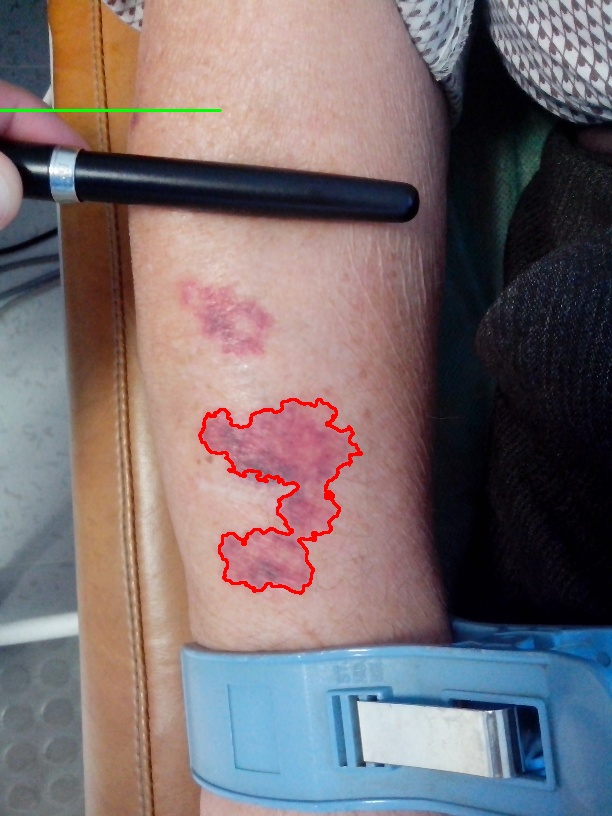
\includegraphics[scale=0.4]{fig/2o.jpeg}
  \caption{Detekcia hematomu.}
  \label{fig:2o}
\end{figure}
\begin{figure}[h]
  \centering
  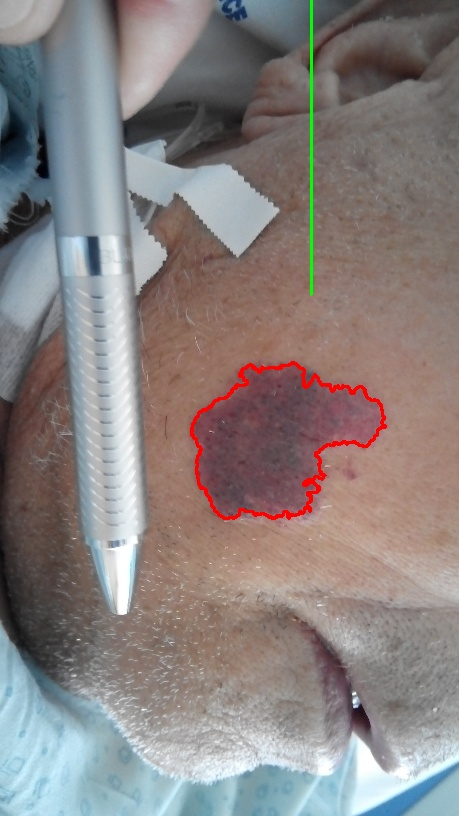
\includegraphics[scale=0.4]{fig/3o.jpeg}
  \caption{Detekcia znamienka.}
  \label{fig:3o}
\end{figure}